\subsection{}
Deux cordes faites d'un même matériau sont attachées ensemble. La deuxième corde (celle de droite) a un diamètre plus grand. Une impulsion se déplace vers la droite dans la première corde, comme sur le schéma suivant :

\begin{center}

\begin{tikzpicture}[scale=0.9]
    \draw[thick] (-3,0) -- (-1.5,0) sin (-1,0.5) cos (-0.5,0) -- (0,0);
    \draw[line width=2.5pt] (0,0) -- (3,0);
    \draw[->, thick] (-1,0.7) -- (-0.5,0.7);
\end{tikzpicture}
\end{center}

Laquelle des images suivantes représente ce qui se passera après que l'impulsion ait atteint le point de jonction entre les deux cordes ?



\begin{center}
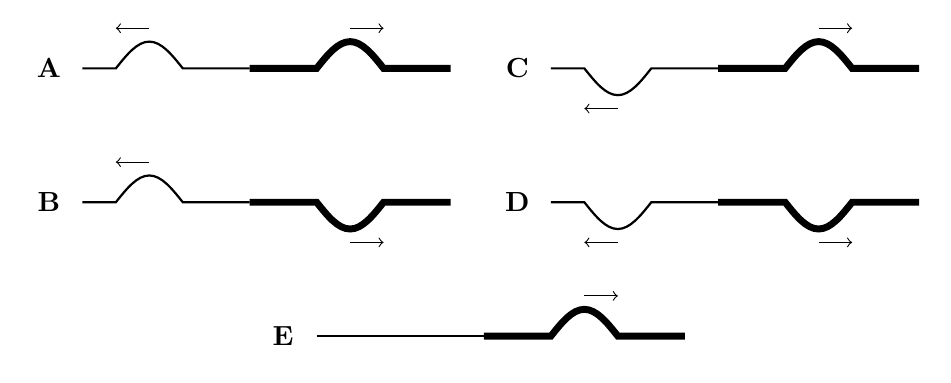
\begin{tikzpicture}[scale=0.85]
    % A
    \node at (-0.5, 3) {\textbf{A}};
    \draw[thick] (0,3) -- (0.5,3) sin (1,3.4) cos (1.5,3) -- (2.5,3);
    \draw[->] (1,3.6) -- (0.5,3.6);
    \draw[line width=2.5pt] (2.5,3) -- (3.5,3) sin (4,3.4) cos (4.5,3) -- (5.5,3);
    \draw[->] (4,3.6) -- (4.5,3.6);

    % C
    \node at (6.5, 3) {\textbf{C}};
    \draw[thick] (7,3) -- (7.5,3) sin (8,2.6) cos (8.5,3) -- (9.5,3);
    \draw[->] (8,2.4) -- (7.5,2.4);
    \draw[line width=2.5pt] (9.5,3) -- (10.5,3) sin (11,3.4) cos (11.5,3) -- (12.5,3);
    \draw[->] (11,3.6) -- (11.5,3.6);

    % B
    \node at (-0.5, 1) {\textbf{B}};
    \draw[thick] (0,1) -- (0.5,1) sin (1,1.4) cos (1.5,1) -- (2.5,1);
    \draw[->] (1,1.6) -- (0.5,1.6);
    \draw[line width=2.5pt] (2.5,1) -- (3.5,1) sin (4,0.6) cos (4.5,1) -- (5.5,1);
    \draw[->] (4,0.4) -- (4.5,0.4);

    % D
    \node at (6.5, 1) {\textbf{D}};
    \draw[thick] (7,1) -- (7.5,1) sin (8,0.6) cos (8.5,1) -- (9.5,1);
    \draw[->] (8,0.4) -- (7.5,0.4);
    \draw[line width=2.5pt] (9.5,1) -- (10.5,1) sin (11,0.6) cos (11.5,1) -- (12.5,1);
    \draw[->] (11,0.4) -- (11.5,0.4);

    % E
    \node at (3, -1) {\textbf{E}};
    \draw[thick] (3.5,-1) -- (6,-1);
    \draw[line width=2.5pt] (6,-1) -- (7,-1) sin (7.5,-0.6) cos (8,-1) -- (9,-1);
    \draw[->] (7.5,-0.4) -- (8,-0.4);
\end{tikzpicture}
\end{center}

\noindent\textbf{Justification :} \hrulefill \\[2.5ex]
\rule{\linewidth}{0.4pt} \\[2.5ex]
\rule{\linewidth}{0.4pt}
\vfill